% !TEX root = ./main.tex
\documentclass[bigger,notes]{beamer}
\usetheme{metropolis}
\title{Bridging the gap between Typestates and Rust in production code}
\author{\textbf{José Duarte}\texorpdfstring{\\ António Ravara (Advisor)}{}}
\date{March 2021}
\institute{NOVA School of Science and Technology}

\usepackage{tikz}
\usetikzlibrary{shapes,backgrounds,positioning}
\usepackage{xcolor}

\usepackage{pgfpages}
\usepackage{hyperref}
% \usepackage{listings}
% \lstset{
%     basicstyle=\small\ttfamily,
%     frame=single,
%     % numberstyle=\tiny,
%     % numbers=left
% }

\usepackage[newfloat]{minted}
\setminted{
    linenos,
    frame=single,
    style=lovelace,
    fontsize=\small,
}

\usepackage[main=american,portuguese]{babel}
\babeltags{pt=portuguese, enUS=american}

\setbeameroption{show notes on second screen}

\begin{document}

\begin{frame}[plain]
    \titlepage

    \note{
        Hello everyone! My name is José Duarte and today I will be talking about using typestates in Rust.
        I'll present:
        \begin{itemize}
            \item A brief definition of typestates.
            \item Why they are useful.
            \item And finally I'll discuss their relationship with Rust and my proposal to integrate them in the ecosystem.
        \end{itemize}
    }
\end{frame}

\AtBeginSection[]
{
    \begin{frame}
        \frametitle{Outline}
        \tableofcontents[currentsection, hideothersubsections]
    \end{frame}
}

\begin{frame}
    \frametitle{Outline}
    \tableofcontents[hideallsubsections]

    \note{
        \begin{pt}
            Durante a apresentação irei introduzir o tema,
            rever sumáriamente o estado da arte,
            apresentar a proposta de trabalho e
            por fim rever o plano de trabalho da mesma.
        \end{pt}
    }
\end{frame}


\section{Introduction}

\subsection{Context}
\begin{frame}
    \frametitle{Context}
    Software plays a crucial role in our lives.
    \begin{itemize}
        \item From web browsers, to word processors and more!
    \end{itemize}

    As software becomes more important, bugs become more expensive.
    \begin{itemize}
        \item Losing work due to a bug in the save procedure is not nice.
        \item A bug in the firmware for a pacemaker may cost a life.
    \end{itemize}
\end{frame}

\subsection{Problem}
\begin{frame}
    \frametitle{Problem}
    \begin{figure}
        \centering
        \begin{tikzpicture}
            \def\X{2}
            \def\fstX{-\X}
            \def\sndX{\X}
            \def\Y{3}
            \def\fstcircle{(\fstX,0) circle (2.5)}
            \def\sndcircle{(\sndX,0) circle (2.5)}

            \begin{scope}[fill opacity=0.35]
                \fill[red] \sndcircle;
                \fill[blue] \fstcircle;
            \end{scope}

            \draw \fstcircle;
            \draw \sndcircle;

            \node at (\fstX, \Y) {Preventable};
            \node at (\sndX, \Y) {Prevented};
        \end{tikzpicture}
        \caption{Diagram of preventable bugs and prevented bugs.}
    \end{figure}
\end{frame}

\begin{frame}
    \frametitle{Problem - with Rust}
    \begin{figure}
        \centering
        \begin{tikzpicture}
            \def\X{1.25}
            \def\fstX{-\X}
            \def\sndX{\X}
            \def\Y{3}
            \def\fstcircle{(\fstX,0) circle (2.5)}
            \def\sndcircle{(\sndX,0) circle (2.5)}

            \begin{scope}[fill opacity=0.35]
                \fill[red] \sndcircle;
                \fill[blue] \fstcircle;
            \end{scope}

            \draw \fstcircle;
            \draw \sndcircle;

            \node at (\fstX, \Y) {Preventable};
            \node at (\sndX, \Y) {Prevented};
        \end{tikzpicture}
        \caption{Diagram of preventable bugs and prevented bugs when considering Rust's borrow checker.}
    \end{figure}
\end{frame}

\begin{frame}
    \frametitle{Problem - Ideal}
    \begin{figure}
        \centering
        \begin{tikzpicture}
            \def\X{0}
            \def\fstX{-\X}
            \def\sndX{\X}
            \def\Y{0}
            \def\fstcircle{(\fstX,0) circle (2.5)}
            \def\sndcircle{(\sndX,0) circle (2.5)}

            \begin{scope}[fill opacity=0.35]
                \fill[red] \sndcircle;
                \fill[blue] \fstcircle;
            \end{scope}

            \draw \fstcircle;
            \draw \sndcircle;

            \node at (\fstX-4, \Y) {Preventable};
            \node at (\sndX+4, \Y) {Prevented};
        \end{tikzpicture}
        \caption{The ideal diagram of preventable bugs and prevented bugs, where all bugs are prevented.}
    \end{figure}
\end{frame}

\subsection{Objectives}
\begin{frame}
    \frametitle{Objectives}

    A library which brings \emph{practical} typestates to Rust.
    \begin{itemize}
        \item Minimal learning overhead.
        \item Zero-cost abstraction.
        \item Scalable to large projects.
    \end{itemize}


\end{frame}

\section{State of the Art}
\subsection{Session Types}
\begin{frame}
    \frametitle{Session Types}

\end{frame}

\subsection{Typestates}
\begin{frame}
    \frametitle{Typestates}

\end{frame}

\section{Case Study}

\subsection{Problem}
\begin{frame}[fragile]
    \frametitle{Problem} % ???
    Error happens at runtime, possibly crashing the program.

    \begin{minted}{Rust}
fn main() {
    let protocol = Protocol::new();
    protocol.step1();
    protocol.step3(); // runtime error
    protocol.step2();
}
    \end{minted}
    Our tools should work for us, not make us work for them.
\end{frame}

\subsection{Solution}
\begin{frame}[fragile]
    \frametitle{Solution}
    Ideally, we want to catch the error at compile-time.
    \begin{minted}{text}
fn main() {
    let protocol = Protocol::new();
    protocol.step1();
    protocol.step3();
             ^^^^^^^
             | error: cannot call `step3`
    protocol.step2();
}
    \end{minted}

\end{frame}

\subsection{Approach}
\begin{frame}
    \frametitle{Approach - Overview}

    We can exploit the Rust typesystem to emulate typestates,
    however this approach requires boilerplate.

    Use macros!
    \begin{itemize}
        \item Integral part of the language, requiring no new experience.
        \item Able to throw errors during compile-time.
        \item Rewrite the annotated code, generating boilerplate for the user.
    \end{itemize}

\end{frame}

\begin{frame}[fragile]
    \frametitle{Approach - Going deeper}

    \begin{figure}
        \centering
        \begin{tikzpicture}
            \tikzstyle{code} = [font=\tiny, align=left]
            \tikzstyle{phase} = [below, font=\small\itshape]

            \def\xSpec{0}
            \def\xAST{4}
            \def\xFSM{8}
            \def\xCode{12}
            \def\yLabel{-1.75}

            \node[code] (code) at (\xSpec,0) {\mintinline{rust}{#[typestate]}\\\mintinline{rust}{// ...}};

            \begin{scope}[shift={(\xAST, 0.75)}]
                \tikzstyle{n}=[circle, draw=blue!70, fill=blue!20]
                \node[n] (root) at (0, 0) {};
                \node[n] (l1) at (-0.35, -0.75) {};
                \node[n] (l2) at (0.35, -0.75) {};
                \node[n] (l11) at (-0.7, -1.5) {};
                \draw[-] (root) -- (l1);
                \draw[-] (root) -- (l2);
                \draw[-] (l1) -- (l11);
            \end{scope}

            \begin{scope}[shift={(\xFSM, 0.75)}]
                \tikzstyle{n}=[circle, draw=blue!70, fill=blue!20]
                \tikzstyle{f}=[circle, draw=red!70, fill=red!20]
                \tikzstyle{s}=[circle, draw=green!70, fill=green!20]
                \node[s] (root) at (0, 0) {};
                \node[n] (l1) at (-0.5, -0.75) {};
                \node[n] (l2) at (0.5, -0.75) {};
                \node[f] (l11) at (0, -1.5) {};
                \draw[->] (root) -- (l1);
                \draw[->] (root) -- (l2);
                \draw[->] (l1) -- (l11);
                \draw[->] (l2) -- (l1);
            \end{scope}

            \node[code] (rust-code) at (\xCode,0) {\mintinline{rust}{struct S { ... }}\\\mintinline{rust}{trait SOps { ... }}\\\mintinline{rust}{// ...}};

            % \draw[->, thick] (code) -> (2.5, 0);
            % \draw[->, thick] (4.5, 0) -> (5, 0);
            % \draw[->, thick] (7, 0) -> (rust-code);

            \node[align=center] (label-1) at (\xSpec, \yLabel) {Typestate\\Specification};
            \node[align=center] (label-2) at (\xAST, \yLabel) {AST};
            \node[align=center] (label-3) at (\xFSM, \yLabel) {State\\Machine};
            \node[align=center] (label-4) at (\xCode, \yLabel) {Rust\\Code};

            \draw[->, thick] (label-1) -- node[phase] {Parse} (label-2);
            \draw[->, thick] (label-2) -- node[phase] {Convert} (label-3);
            \draw[->, thick] (label-3) -- node[phase] {Check: Ok} (label-4);
            \draw[->, thick] (label-3) edge[in=-35, out=-145] node[phase] {Check: Error} (label-1);

        \end{tikzpicture}
    \end{figure}

\end{frame}

\subsection{Workflow}
\begin{frame}[fragile]
    \frametitle{Workflow - Design the state machine}
    Consider a traffic light as a state machine.
    \begin{figure}
        \centering
        \begin{tikzpicture}
            \node[circle, thick, minimum size=0.75cm, draw=green!70, fill=green!30] (g) at (0, 0) {};
            \node[circle, thick, minimum size=0.75cm, draw=yellow, fill=yellow!50] (y) at (4, 0) {};
            \node[circle, thick, minimum size=0.75cm, draw=red!70, fill=red!30] (r) at (8, 0) {};
            \node[circle, thick, minimum size=0.6cm, draw=red!70, fill opacity=0] at (8, 0) {};
            \draw[->, very thick, draw=black!70] (g) -- node[above, font=\small\ttfamily] {to\_yellow} (y);
            \draw[->, very thick, draw=black!70] (y) -- node[above, font=\small\ttfamily] {to\_red} (r);
            \draw[->, very thick, draw=black!70] (r) edge[in=-30, out=-150] node[above, font=\small\ttfamily] {to\_green} (g);
            \draw[->, very thick, draw=black!70] (8, 1) -- node[right, font=\small\ttfamily] {turn\_on} (r);
            \draw[->, very thick, draw=black!70] (r) edge[loop below] node[below, font=\small\ttfamily] {turn\_off} (r);
        \end{tikzpicture}
    \end{figure}
\end{frame}

\begin{frame}[fragile]
    \frametitle{Workflow - Declaring state in Rust}
    Using the DSL we first declare the module, main automata and the states:
    \begin{listing}
        \centering
        \begin{minted}{rust}
#[typestate] mod traffic_light {
    #[automata] struct TrafficLight;
    #[state] struct Green;
    #[state] struct Yellow;
    #[state] struct Red;
    // ...
        \end{minted}
    \end{listing}
    We still need transitions!
\end{frame}

\begin{frame}[fragile]
    \frametitle{Workflow - Declaring transitions in Rust}
    All transition functions take ownership of the current state and return the new state.
    \begin{listing}
        \centering
        \begin{minted}{rust}
    // code from the previous slide ...
    fn to_yellow(self: Green) -> Yellow;
    fn to_red(self: Yellow) -> Red;
    fn to_green(self: Red) -> Green;
    // ...
        \end{minted}
    \end{listing}
    Finally, we need \emph{start} and \emph{end} states.
\end{frame}

\begin{frame}[fragile]
    \frametitle{Workflow - Declaring \emph{start} and \emph{end} states in Rust}
    Functions that do not use \texttt{self} and \emph{return} a valid state are inferred as the \emph{start} state.

    Functions that take \texttt{self} and do \emph{not return }a valid state are inferred as the \emph{end} state.
    \begin{listing}
        \centering
        \begin{minted}{rust}
    // code from the previous slides ...
    fn turn_on() -> Red;
    fn turn_off(self: Red);
}
        \end{minted}
    \end{listing}
    Our traffic light is ready!
\end{frame}

\begin{frame}[fragile]
    \frametitle{Workflow - The other features}
    There are still other important features left.
    For maintenance purposed, consider that our traffic light is now required to count every \texttt{GYR} cycle. % Green->Yellow->Red

    The \texttt{TrafficLight} structure is now declared as follows:
    \begin{listing}
    \centering
        \begin{minted}{rust}
#[automata] struct TrafficLight { cycles:u64 }
        \end{minted}
    \end{listing}
\end{frame}

\begin{frame}[fragile]
    \frametitle{Workflow - The other features}
    How can we check if the light requires maintenance?

    We add a \texttt{pure} function:
    \begin{listing}
    \centering
        \begin{minted}{rust}
fn requires_maintenance(
    &self: TrafficLight
) -> bool;
        \end{minted}
    \end{listing}
    This function is not able to perform mutations due to the immutable reference (\texttt{\&}).
\end{frame}

\begin{frame}[fragile]
    \frametitle{Workflow - The other features}
    How can we check if the light requires maintenance?

    We add a \texttt{pure} function:
    \begin{listing}
    \centering
        \begin{minted}{rust}
fn requires_maintenance(
    self: &TrafficLight
) -> bool;
        \end{minted}
    \end{listing}
    This function is not able to perform mutations due to the immutable reference (\texttt{\&}).
\end{frame}

\begin{frame}[fragile]
    \frametitle{Workflow - The other features}
    After maintenance, how can we reset the counter?

    We add an \texttt{impure} function:
    \begin{listing}
    \centering
        \begin{minted}{rust}
fn reset_counter(self: &mut TrafficLight);
        \end{minted}
    \end{listing}
    The function is able to perform mutations, due to usage of a mutable reference (\texttt{\&mut}),
    but it is unable to transition between states.
\end{frame}

\section{Plan}

\begin{frame}
    \frametitle{Plan Overview}

    \begin{figure}[h]
        \centering
        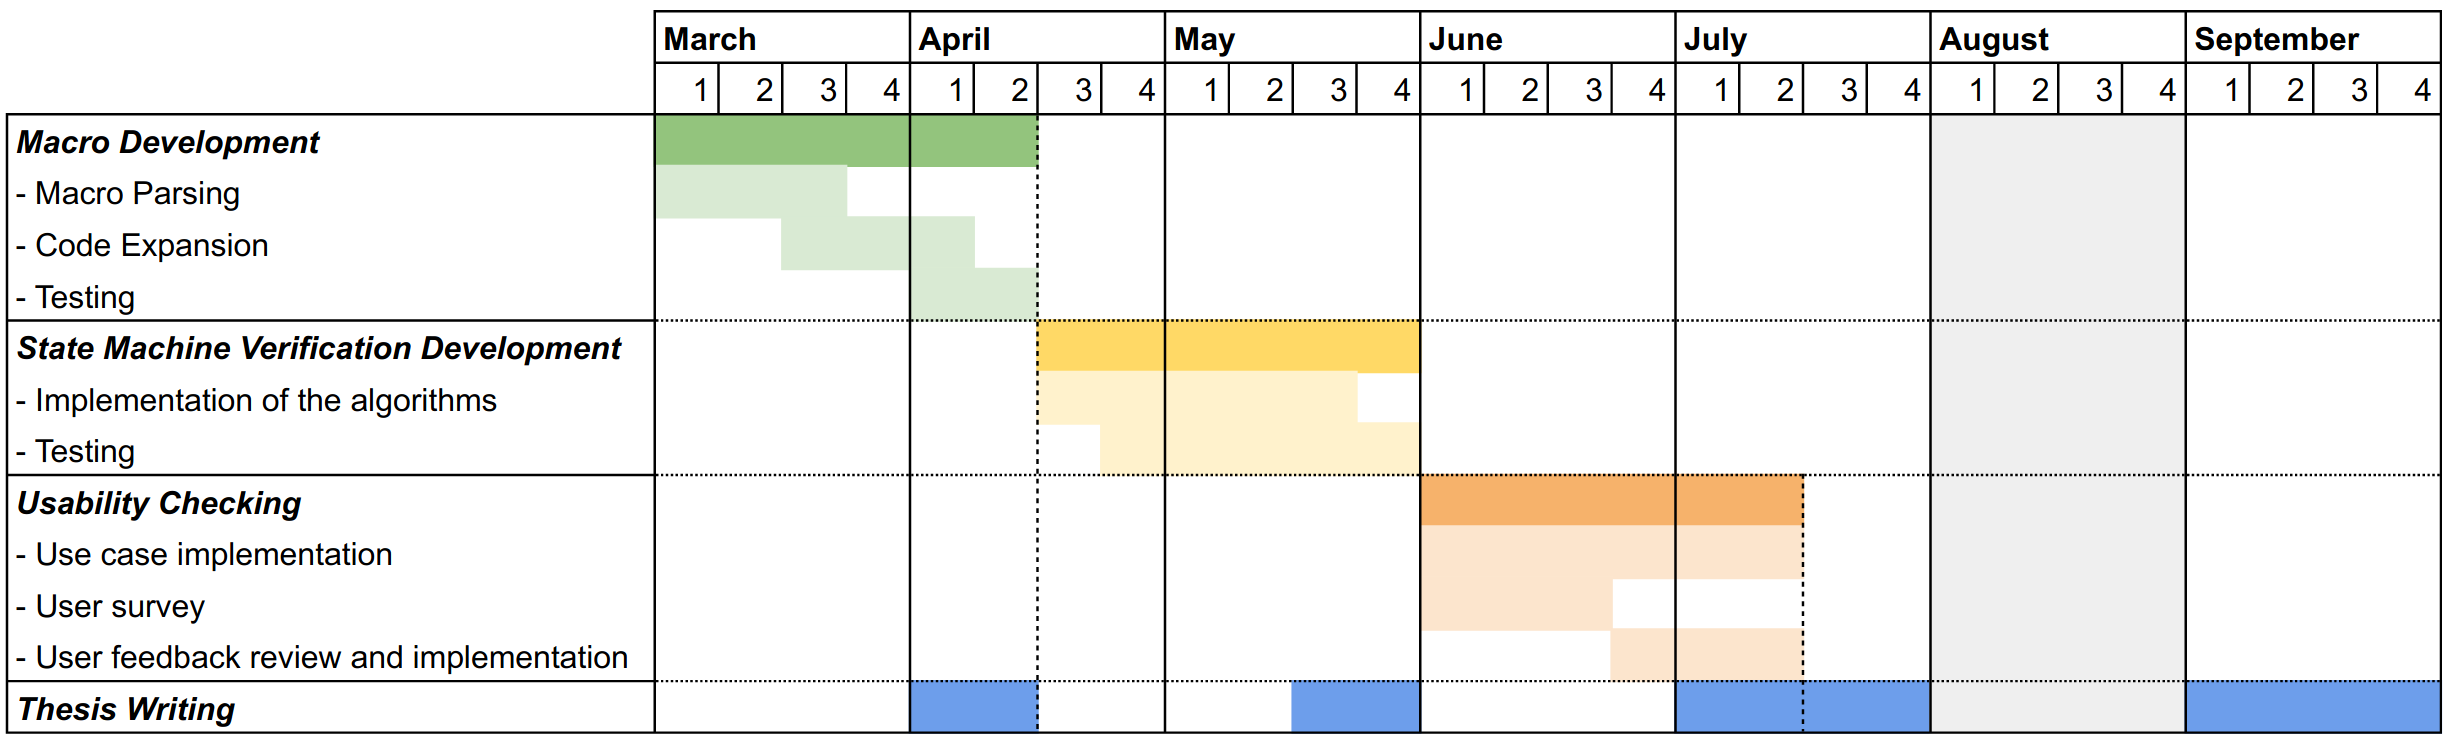
\includegraphics[width=\linewidth]{planning.png}
        \caption{Work plan Gantt chart}
    \end{figure}

\end{frame}

\end{document}